% !TEX root = ../thesis.tex

\section{Results}
\label{sec:results}
This is the Results section.

\subsection{SOM Metrics}
\label{subsec:results_som_metrics}

\subsubsection{SOM-Induced Quantization}
\label{subsubsec:results_som_quantization}

heat map showing distance?

\subsubsection{Vector-Node Count}
\label{subsubsec:results_vector_node_count}

\subsubsection{Map Emptiness}
\label{subsubsec:results_map_emptiness}

\begin{figure}[!htb]
  \centering
\begin{subfigure}{0.45\textwidth}
  \centering
  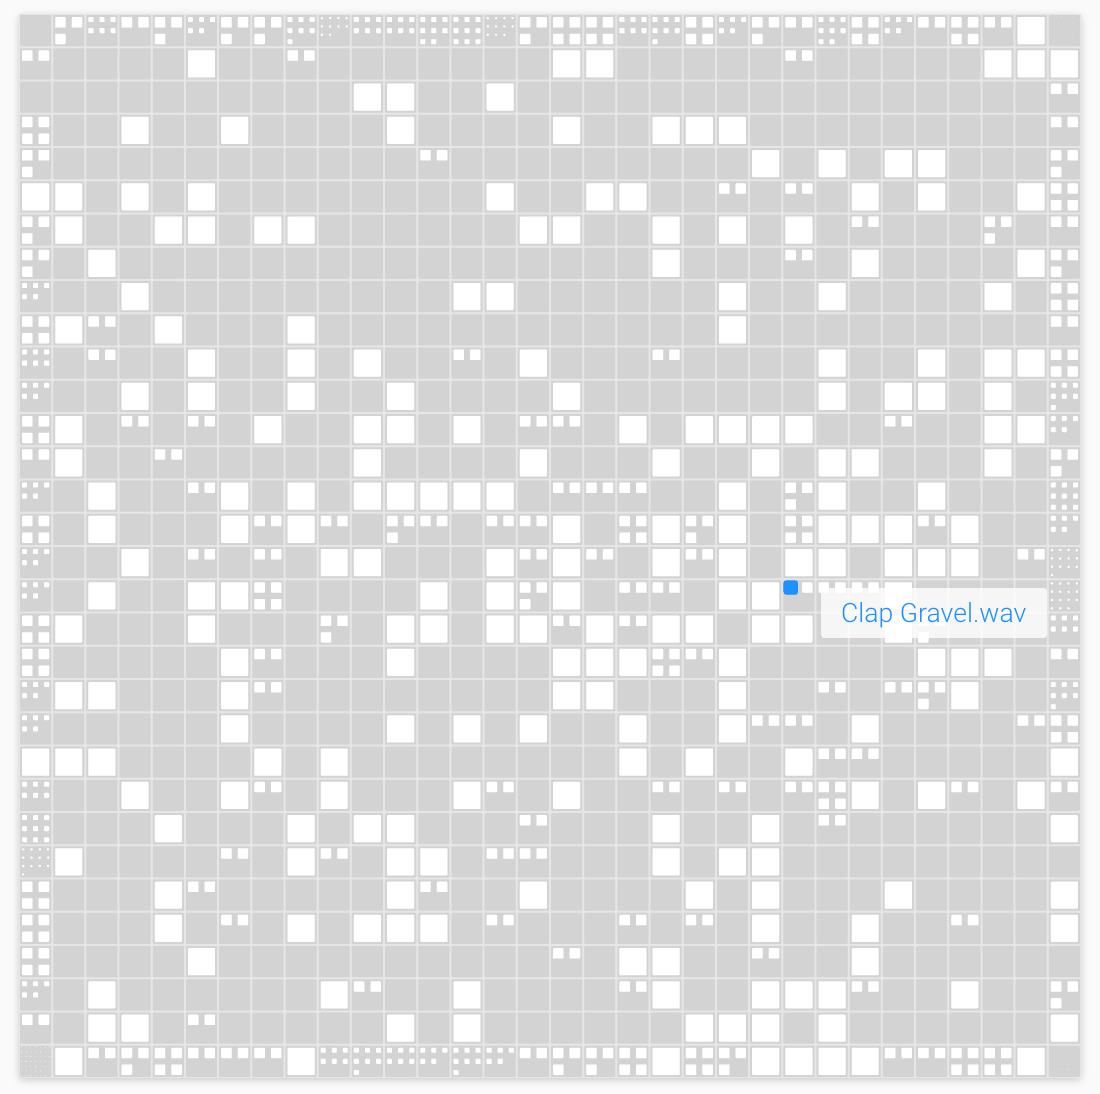
\includegraphics[width=\textwidth]{SOM-Browser_no-FNP}
  \caption{\textit{SOM Browser} without \gls{fnp}}
  \label{fig:results_no_fnp}
\end{subfigure}
~
\begin{subfigure}{0.45\textwidth}
  \centering
  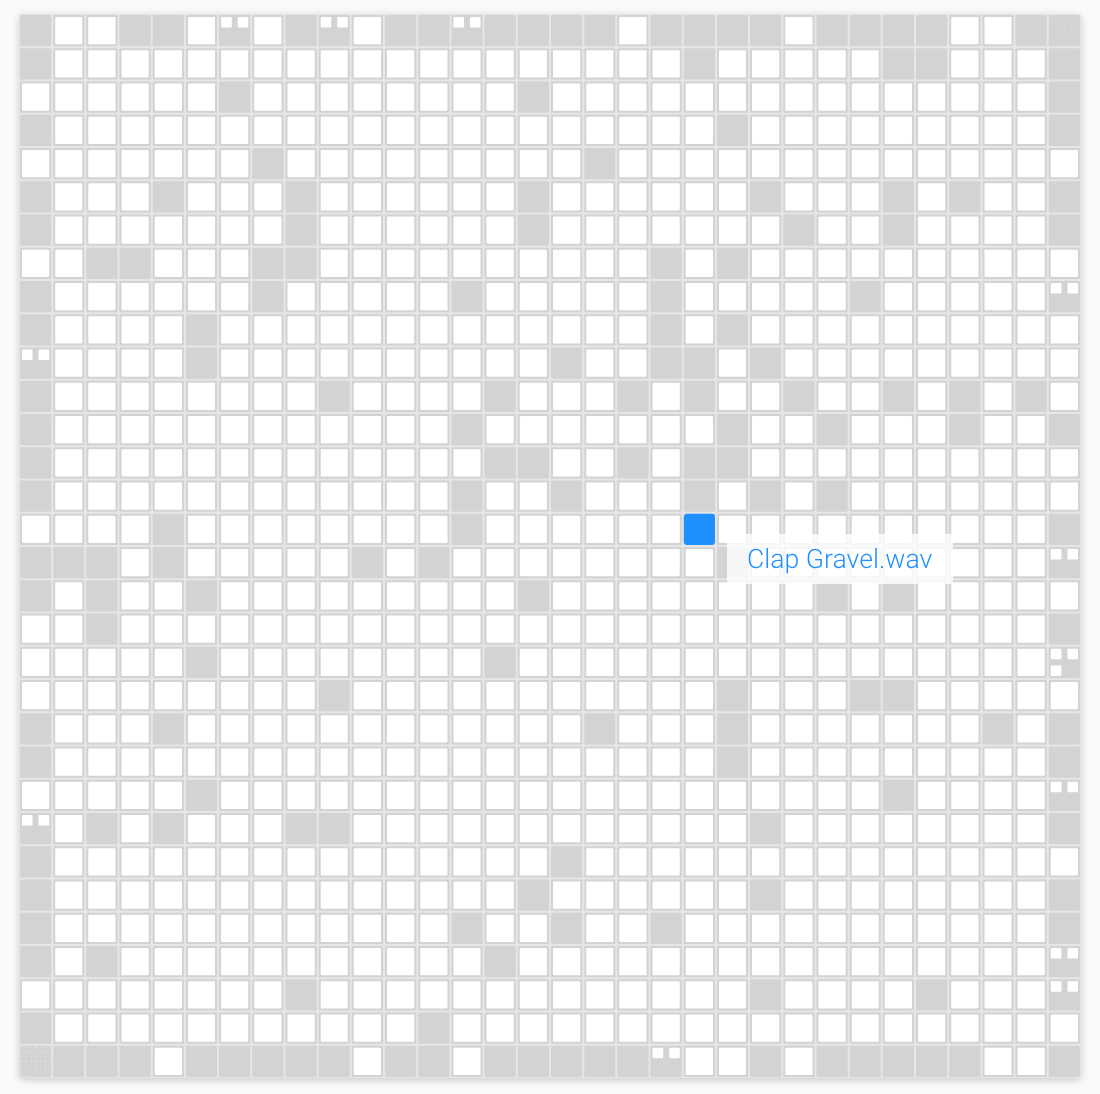
\includegraphics[width=\textwidth]{SOM-Browser_FNP}
  \caption{\textit{SOM Browser} with \gls{fnp}}
  \label{fig:results_fnp}
\end{subfigure}
\caption[\textit{SOM Browser}: Influence of FNP on Map Emptiness]
{\textit{SOM Browser}: Influence of FNP on Map Emptiness for the
\textit{Drum Essentials} sample library}
\label{fig:results_fnp_comparison}
\end{figure}


\subsection{Interview Results}
\label{subsec:results_interview}

Reference grounded theory?

code categories: cognitive, physical, perceptual, strategies, interaction style

phys: arrow keys

perceptual: colors, font size, map order

cognitive: map order, no labelled axes, overwhelming / clear interface

emergent coding vs a priori

Overview Code Tree?

\begin{figure}[!htb]
  \centering
\Tree[.IP [.NP [.Det \textit{the} ]
               [.N\1 [.N \textit{package} ]]]
          [.I\1 [.I \textsc{3sg.Pres} ]
                [.VP [.V\1 [.V \textit{is} ]
                           [.AP [.Deg \textit{really} ]
                                [.A\1 [.A \textit{simple} ]
                                      \qroof{\textit{to use}}.CP ]]]]]]
\caption{A tree caption}
\label{table:tree_test}
\end{figure}

cite \citet{saldana2015}

\begin{figure}[!htb]
  \centering
  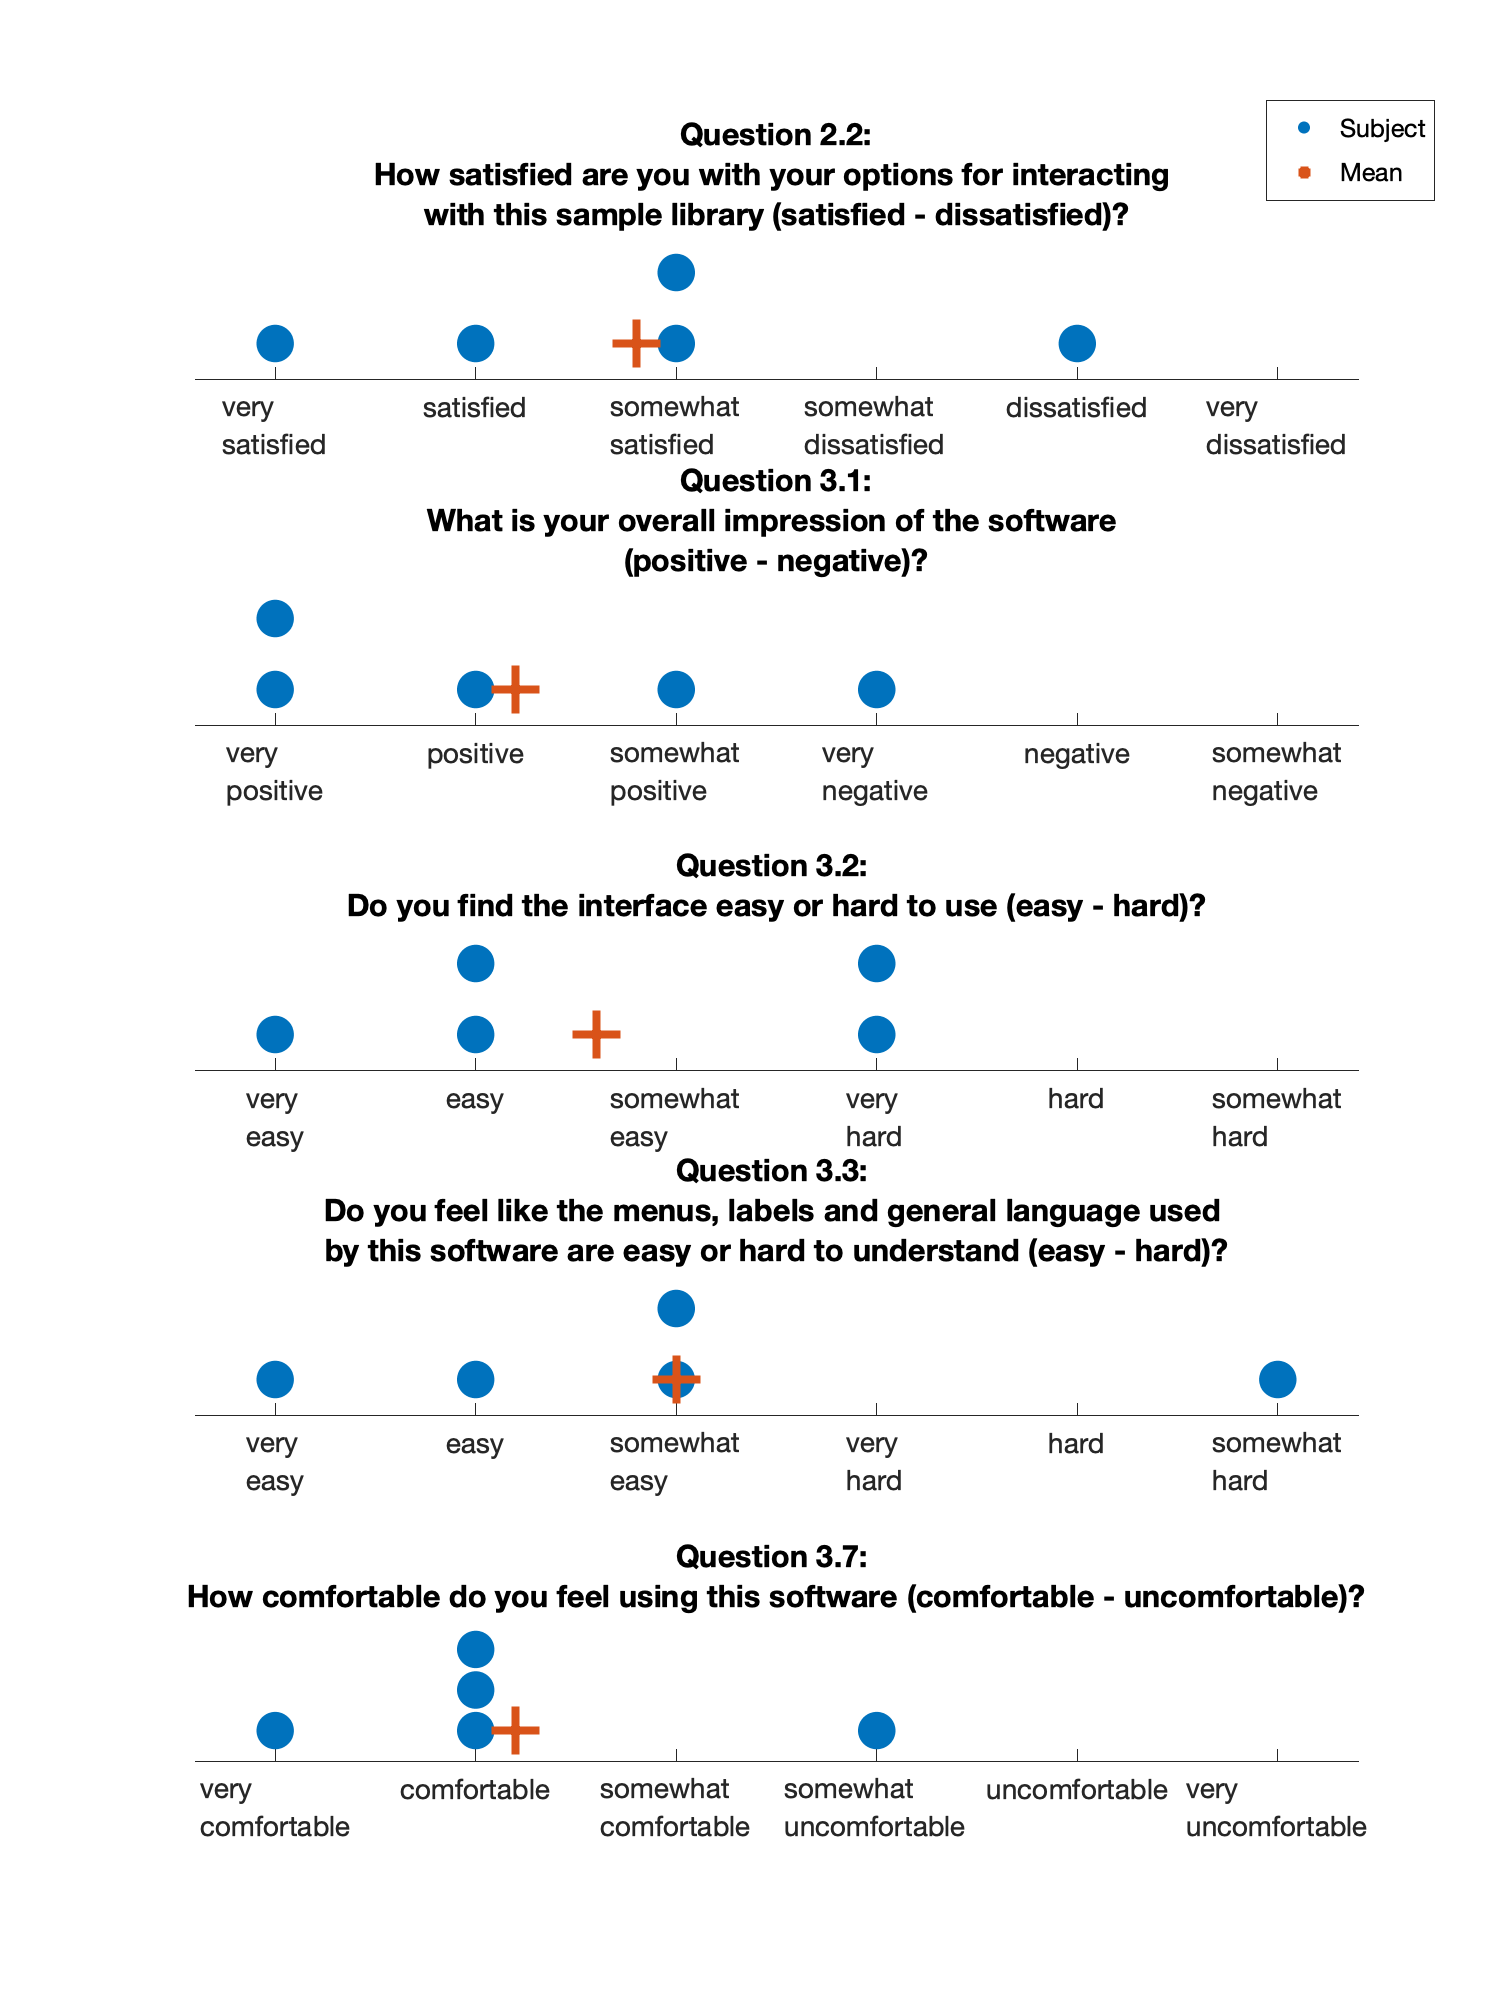
\includegraphics[width=\linewidth, trim = 25mm 10mm 10mm 10mm, clip]
  {eval_ratings}
  \caption[Interview Ratings]{Likert scale ratings by interview subjects for
  questions concerning satisfaction with their current sample library workflow
  and first \textit{SOM Browser} impressions}
  \label{fig:results_ratings}
\end{figure}

\clearpage

\begin{table}[!htb]
  \renewcommand{\arraystretch}{1.2}
  \centering
  \footnotesize
  % \rowcolors{2}{table-bg-one}{table-bg-two}
  \begin{tabular}{ p{3.5cm} p{5cm} p{5cm} }
  \multicolumn{3}{ l }{\textbf{Question 2.1:}} \\
  \multicolumn{3}{ p{14.5cm} }{\textbf{Imagine you were asked to familiarize
  yourself with the presented sample library in order to use it in some of your
  work. Can you describe how you would approach this task?}} \\
  \hline
    \textbf{Code} & \textbf{Example} & \textbf{Summary} \\
    \hline
    \textbf{Mental Representation}
    &
    "I know exactly what I'm looking for"
    &
    Subjects often have a clear \textbf{mental representation} of the sound they
    are searching.
    \\

    \textbf{Goal Pursuit}
    &
    [I listen to sounds] "[u]ntil I find the one that I want"
    &
    Subjects will only look for sounds until they find something that satisfies
    their immediate needs.
    \\
    \textbf{Iteration}
    &
    "I will have like eight different kick drums [...] and then I go through
    them again as another iteration of choice."
    &
    Subjects will select a variety of samples as potential candidates and then
    perform another search among the selected subset.
    \\
    \textbf{Frustration}
    &
    "it takes a lot of time actually and it's not the most fun part"
    &
    Looking through lists of samples sequentially is perceived to cause
    \textbf{frustration}.
    \\
  \end{tabular}
  \caption[Question 2.1: Response codes]{Question 2.1: Response codes with
  example data and interpretive summary}
  \label{table:responses_question_2-1}
\end{table}

\begin{table}[!ht]
  \renewcommand{\arraystretch}{1.2}
  \centering
  \footnotesize
  % \rowcolors{2}{table-bg-one}{table-bg-two}
  \begin{tabular}{ p{3.5cm} p{5cm} p{5cm} }
  \multicolumn{3}{ l }{\textbf{Question 2.2:}} \\
  \multicolumn{3}{ p{14.5cm} }{\textbf{How satisfied are you with your options
  for interacting with this sample library?}} \\
  \hline
    \textbf{Code} & \textbf{Example} & \textbf{Summary} \\
    \hline
    \textbf{Example}
    &
    "Here's an example of something someone said."
    &
    Subjects said this because they believe it to be true.
    \\
  \end{tabular}
  \caption[Question 2.2: Response codes]{Question 2.2: Response codes with
  example data and interpretive summary}
  \label{table:responses_question_2-2}
\end{table}

\begin{table}[!ht]
  \renewcommand{\arraystretch}{1.2}
  \centering
  \footnotesize
  % \rowcolors{2}{table-bg-one}{table-bg-two}
  \begin{tabular}{ p{3.5cm} p{5cm} p{5cm} }
  \multicolumn{3}{ l }{\textbf{Question 3.1:}} \\
  \multicolumn{3}{ p{14.5cm} }{\textbf{What is your overall impression of the
  software (positive - negative)? What do you think works or doesn’t work?}} \\
  \hline
    \textbf{Code} & \textbf{Example} & \textbf{Summary} \\
    \hline
    \textbf{Example}
    &
    "Here's an example of something someone said."
    &
    Subjects said this because they believe it to be true.
    \\
  \end{tabular}
  \caption[Question 3.1: Response codes]{Question 3.1: Response codes with
  example data and interpretive summary}
  \label{table:responses_question_3-1}
\end{table}

\begin{table}[!ht]
  \renewcommand{\arraystretch}{1.2}
  \centering
  \footnotesize
  % \rowcolors{2}{table-bg-one}{table-bg-two}
  \begin{tabular}{ p{3.5cm} p{5cm} p{5cm} }
  \multicolumn{3}{ l }{\textbf{Question 3.2:}} \\
  \multicolumn{3}{ p{14.5cm} }{\textbf{Do you find the interface easy or hard to
  use (easy - hard)? Can you elaborate on why?}} \\
  \hline
    \textbf{Code} & \textbf{Example} & \textbf{Summary} \\
    \hline
    \textbf{Example}
    &
    "Here's an example of something someone said."
    &
    Subjects said this because they believe it to be true.
    \\
  \end{tabular}
  \caption[Question 3.2: Response codes]{Question 3.2: Response codes with example
  data and interpretive summary}
  \label{table:responses_question_3-2}
\end{table}

\begin{table}[!ht]
  \renewcommand{\arraystretch}{1.2}
  \centering
  \footnotesize
  % \rowcolors{2}{table-bg-one}{table-bg-two}
  \begin{tabular}{ p{3.5cm} p{5cm} p{5cm} }
  \multicolumn{3}{ l }{\textbf{Question 3.3:}} \\
  \multicolumn{3}{ p{14.5cm} }{\textbf{Do you feel like the menus, labels and
  general language used by this software are easy or hard to understand
  (easy - hard)?}} \\
  \hline
    \textbf{Code} & \textbf{Example} & \textbf{Summary} \\
    \hline
    \textbf{Example}
    &
    "Here's an example of something someone said."
    &
    Subjects said this because they believe it to be true.
    \\
  \end{tabular}
  \caption[Question 3.3: Response codes]{Question 3.3: Response codes with
  example data and interpretive summary}
  \label{table:responses_question_3-3}
\end{table}

\begin{table}[!ht]
  \renewcommand{\arraystretch}{1.2}
  \centering
  \footnotesize
  % \rowcolors{2}{table-bg-one}{table-bg-two}
  \begin{tabular}{ p{3.5cm} p{5cm} p{5cm} }
  \multicolumn{3}{ l }{\textbf{Question 3.4:}} \\
  \multicolumn{3}{ p{14.5cm} }{\textbf{What do you think about the organization
  of sounds in this interface?}} \\
  \hline
    \textbf{Code} & \textbf{Example} & \textbf{Summary} \\
    \hline
    \textbf{Example}
    &
    "Here's an example of something someone said."
    &
    Subjects said this because they believe it to be true.
    \\
  \end{tabular}
  \caption[Question 3.4: Response codes]{Question 3.4: Response codes with
  example
  data and interpretive summary}
  \label{table:responses_question_3-4}
\end{table}

\begin{table}[!ht]
  \renewcommand{\arraystretch}{1.2}
  \centering
  \footnotesize
  % \rowcolors{2}{table-bg-one}{table-bg-two}
  \begin{tabular}{ p{3.5cm} p{5cm} p{5cm} }
  \multicolumn{3}{ l }{\textbf{Question 3.5:}} \\
  \multicolumn{3}{ p{14.5cm} }{\textbf{What do you think the axes represent?}} \\
  \hline
    \textbf{Code} & \textbf{Example} & \textbf{Summary} \\
    \hline
    \textbf{Example}
    &
    "Here's an example of something someone said."
    &
    Subjects said this because they believe it to be true.
    \\
  \end{tabular}
  \caption[Question 3.5: Response codes]{Question 3.2: Response codes with
  example data and interpretive summary}
  \label{table:responses_question_3-5}
\end{table}

\begin{table}[!ht]
  \renewcommand{\arraystretch}{1.2}
  \centering
  \footnotesize
  % \rowcolors{2}{table-bg-one}{table-bg-two}
  \begin{tabular}{ p{3.5cm} p{5cm} p{5cm} }
  \multicolumn{3}{ l }{\textbf{Question 3.6:}} \\
  \multicolumn{3}{ p{14.5cm} }{\textbf{Which do you prefer: the map layout or a
  traditional file manager interface and folder structure (or a combination of
  both)?}} \\
  \hline
    \textbf{Code} & \textbf{Example} & \textbf{Summary} \\
    \hline
    \textbf{Example}
    &
    "Here's an example of something someone said."
    &
    Subjects said this because they believe it to be true.
    \\
  \end{tabular}
  \caption[Question 3.6: Response codes]{Question 3.6: Response codes with
  example data and interpretive summary}
  \label{table:responses_question_3-6}
\end{table}

\begin{table}[!ht]
  \renewcommand{\arraystretch}{1.2}
  \centering
  \footnotesize
  % \rowcolors{2}{table-bg-one}{table-bg-two}
  \begin{tabular}{ p{3.5cm} p{5cm} p{5cm} }
  \multicolumn{3}{ l }{\textbf{Question 3.7:}} \\
  \multicolumn{3}{ p{14.5cm} }{\textbf{How comfortable do you feel using this
  software (comfortable - uncomfortable)?}} \\
  \hline
    \textbf{Code} & \textbf{Example} & \textbf{Summary} \\
    \hline
    \textbf{Example}
    &
    "Here's an example of something someone said."
    &
    Subjects said this because they believe it to be true.
    \\
  \end{tabular}
  \caption[Question 3.7: Response codes]{Question 3.7: Response codes with
  example data and interpretive summary}
  \label{table:responses_question_3-7}
\end{table}

\begin{table}[!ht]
  \renewcommand{\arraystretch}{1.2}
  \centering
  \footnotesize
  % \rowcolors{2}{table-bg-one}{table-bg-two}
  \begin{tabular}{ p{3.5cm} p{5cm} p{5cm} }
  \multicolumn{3}{ l }{\textbf{Question 3.8:}} \\
  \multicolumn{3}{ p{14.5cm} }{\textbf{Would you consider using this tool in the
  future or not? If not, what changes would you like to see?}} \\
  \hline
    \textbf{Code} & \textbf{Example} & \textbf{Summary} \\
    \hline
    \textbf{Example}
    &
    "Here's an example of something someone said."
    &
    Subjects said this because they believe it to be true.
    \\
  \end{tabular}
  \caption[Question 3.8: Response codes]{Question 3.8: Response codes with
  example data and interpretive summary}
  \label{table:responses_question_3-8}
\end{table}
